\documentclass[9pt]{beamer}
\usepackage[UTF8]{ctex}

\usepackage{xcolor}
\usepackage{layouts}
\usepackage{minted}
\usepackage[most]{tcolorbox}
\tcbuselibrary{minted}
\usepackage{booktabs}
\usepackage{outlines}
\usepackage{hyperref}
\usepackage{graphicx}
\beamertemplatenavigationsymbolsempty
\usepackage{fontspec}
\setmonofont{Fira Code}[Contextuals=Alternate]


\AtBeginSection[]{
  \begin{frame}
  \tableofcontents[currentsection, hideothersubsections]
  \end{frame}
}

% color
\definecolor{coreFontMain}{RGB}{26,26,26}
\definecolor{coreFontSub}{RGB}{106,106,106}
\definecolor{coreBackgroundLight}{RGB}{230,230,230}
\definecolor{coreBackground}{RGB}{255,255,255}

% heading
\newlength{\headerheight}
\setlength{\headerheight}{0.094\paperheight}


\setbeamerfont{frametitle}{size=\fontsize{12}{14.4}}
\setbeamertemplate{frametitle}
{%
\nointerlineskip
\begin{beamercolorbox}[wd=\paperwidth,left,sep=0pt]{}
\begin{tcolorbox}[enhanced,frame hidden, 
    borderline south={0.5pt}{0pt}{coreFontSub},
    colback=coreBackground, coltext=coreFontSub,height=\headerheight,notitle,left*=0.05\paperwidth,boxsep=0pt,bottom=0pt,halign=left,valign=bottom,before skip=0pt,after skip=0pt, before upper=\strut]
    \usebeamercolor{frametitle}\insertframetitle
\end{tcolorbox}
\end{beamercolorbox}
}


% footer
\newlength{\footerheight}
\setlength{\footerheight}{0.04\paperheight}
\setbeamercolor{footer}{bg=coreBackgroundLight, fg=coreFontMain}

\setbeamertemplate{footline}
{%
\begin{beamercolorbox}[sep=0pt,wd=\paperwidth,center]{footer}
\begin{minipage}[c][\footerheight]{\textwidth}
    \centering
    \insertframenumber/\inserttotalframenumber
\end{minipage}
\end{beamercolorbox}
}



% Title Page

% header
\newlength{\titleheaderheight}
\setlength{\titleheaderheight}{0.0666667\paperheight}
\setbeamercolor{header}{bg=coreBackgroundLight}

%% logo
\newlength{\logoheight}
\setlength{\logoheight}{0.297\paperheight}

%% title
\setbeamercolor{title}{fg=coreFontMain}
\setbeamerfont{title}{size=\fontsize{18.14}{21.768}}
\newlength{\titleheight}
\setlength{\titleheight}{0.19\paperheight}


%% meta
\newlength{\metaheight}
\setlength{\metaheight}{0.21\paperheight}
\setbeamercolor{meta}{fg=coreFontSub}
\setbeamerfont{meta}{size=\fontsize{9.07}{10.884}}

%% contact
\newlength{\contactheight}
\setlength{\contactheight}{0.193333\paperheight}



\setbeamertemplate{title page}{
\nointerlineskip
\begin{beamercolorbox}[wd=\paperwidth,ht=\titleheaderheight]{header}
\end{beamercolorbox}
\nointerlineskip
\begin{beamercolorbox}[wd=\paperwidth,ht=\logoheight]{}
\end{beamercolorbox}
\nointerlineskip
\begin{tcolorbox}[enhanced,frame hidden, borderline south={0.5pt}{0pt}{coreFontMain}, colback=coreBackground,height=\titleheight,boxsep=0pt,bottom=20pt,notitle,halign=flush center,valign=center,before skip=0pt,after skip=0pt, coltext=coreFontMain]
\usebeamercolor{title}
\usebeamerfont{title}\inserttitle

\end{tcolorbox}

\usebeamercolor[fg]{meta}{
\begin{minipage}[c][\metaheight]{\textwidth}
    \centering
    \insertauthor \linebreak
    \insertinstitute \linebreak
    \insertdate
\end{minipage}
}


\begin{tcolorbox}[enhanced,frame hidden, colback=coreBackground,height=\contactheight,notitle,halign=flush center,valign=top,before skip=0pt,after skip=0pt,top=-5pt]
\begin{tabular}{ccc}

\includegraphics[height=3mm]{bohanbeamerstyle/figures/mail.png} & 
\includegraphics[height=3mm]{bohanbeamerstyle/figures/github.png} &
\includegraphics[height=3mm]{bohanbeamerstyle/figures/Twitter.png}
\end{tabular}

\end{tcolorbox}




\begin{beamercolorbox}[sep=2pt,center,wd=\paperwidth,ht=\footerheight]{footer}
\tiny
\insertframenumber/\inserttotalframenumber
\end{beamercolorbox}
\nointerlineskip
}


% 
\setbeamercolor{normal text}{bg=coreBackground,fg=coreFontMain}

% itemize
\setbeamertemplate{itemize items}[circle]

\setlength{\leftmarginii}{10pt}
\setbeamercolor{itemize item}{fg=coreFontMain}
\setbeamercolor{itemize subitem}{fg=coreFontMain}
\setbeamercolor{itemize subsubitem}{fg=coreFontMain}



% code

\newtcblisting{codebox}[2]{listing only, title={#2}, minted language={#1}, minted style=xcode, minted options={fontsize=\fontsize{8}{9.6}, fontfamily=tt}, left=3mm}

\title{网页爬虫简介}
\author{张博涵}
\institute{北京航空航天大学}
\date{\today}

\begin{document}

\begin{frame}[plain]
\maketitle
\end{frame}


\begin{frame}
    \frametitle{Contents}

    \tableofcontents

\end{frame}


\section{网站的基本知识}

\begin{frame}
    \frametitle{网站构成}

互联网上的网站一般有如下构成:

\begin{itemize}
    \item 域名
    \item 服务端与客户端
    \item 网页与相关资源
    \item ...
\end{itemize}




\end{frame}


\begin{frame}
    \frametitle{TCP/IP协议与DNS解析}

    \begin{block}{TCP/IP协议:互联网数据传输规范}
        \begin{itemize}
            \item 互联网上服务器/客户端都有IP地址,该地址由TCP/IP协议规定,主要有IPv4(目前最广泛)以及IPv6(未来的趋势)
            \item 为了对网络进行划分,一般会区分局域网(LAN)以及广域网(WAN),例如家里的一个路由器以及连接在路由器上的设备可以构成一个局域网。
            \item IPv4地址由4个0-255的整数构成,例如\mintinline{shell}{192.168.1.1}通常是局域网中的路由器的地址,\mintinline{shell}{144.144.144.144}是一个常用的DNS解析服务器地址。
        \end{itemize}
    \end{block}
    
    \begin{block}{域名与DNS解析}
\begin{itemize}
    \item 域名是为了让网站更有辨识度而发明的一种,主要格式为xxx.xxx.xxx.xxx,例如 accounts.google.com
    \item 域名从后往前,以.区分,依次为一级域名、二级域名、三级域名...,二级域名可以自由申请注册。一级域名如 .com, .cn, .me等。
    \item DNS解析的主要目的是从域名向IP地址进行映射。
    \item 在访问某个网页时,客户端会首先向DNS服务器进行请求,获取域名的IP地址,然后根据TCP/IP协议进行数据的传输。
\end{itemize}
    \end{block}



\end{frame}


\begin{frame}
    \frametitle{HTTP协议}

    \begin{itemize}
        \item HTTP协议规定了互联网上传输的数据如何包装,现在主要包括HTTP、以及HTTPS
        \item HTTPS = SSL + HTTP,对HTTP请求进行了加密,更安全。
        \item 客户端在访问网页时,会向服务端发送HTTP请求(HTTP request),服务端会进行回应(HTTP response)。
    \end{itemize}

   \begin{figure}
    \centering
    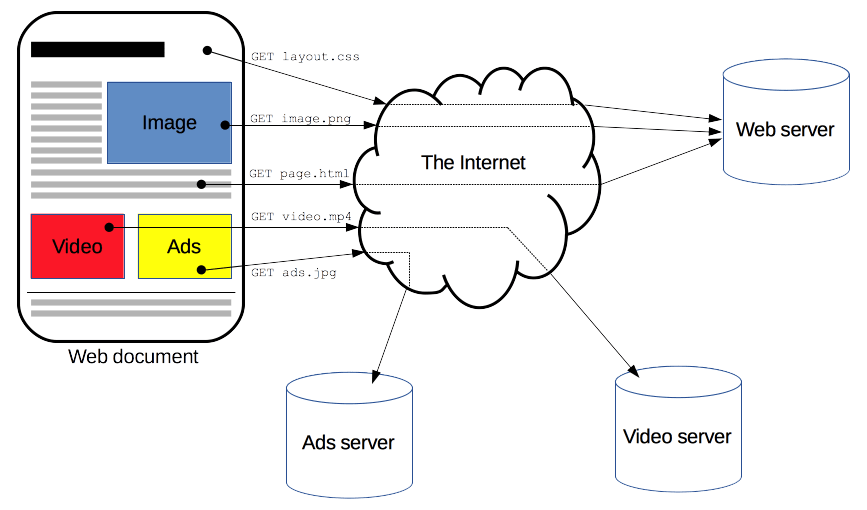
\includegraphics[height=0.5\paperheight]{figures/fetching_a_page.png}
   \end{figure}

\end{frame}

\begin{frame}
    \frametitle{HTTP Request}
    \begin{figure}
        \centering
        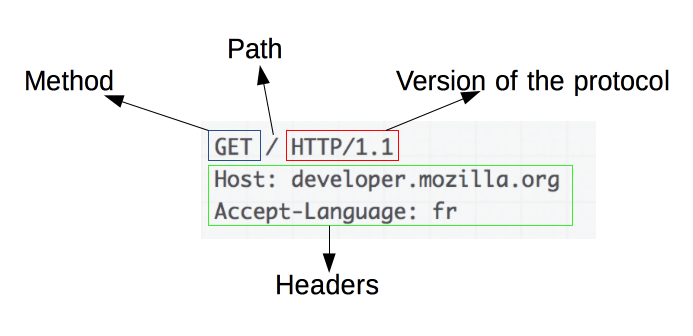
\includegraphics[height=0.5\paperheight]{figures/http_request.png}
       \end{figure}

\begin{itemize}
\item method: HTTP请求的方法,有GET、POST、PUT、DELETE等,主要取决于你在做什么操作
\item path: 请求的相对于Host的路径
\item headers: 请求头,一些辅助信息,如User-Agent可以用于描述当前浏览器的信息
\item body: 请求体,在POST之类的方法中存在,主要用于向服务器提交数据。
\end{itemize}
\end{frame}




\begin{frame}
\frametitle{HTTP Response}
\begin{figure}
\centering
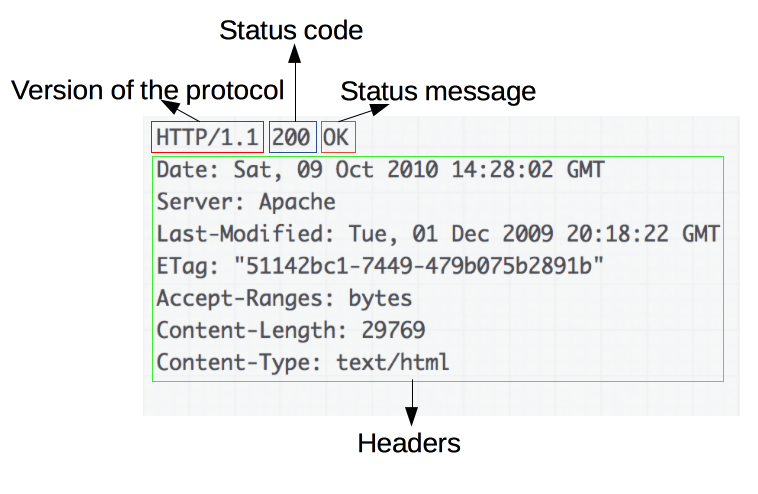
\includegraphics[height=0.5\paperheight]{figures/http_response.png}
\end{figure}

\begin{itemize}
    \item status code: 状态码
    \item headers: 响应头,包含一些响应相关的信息
    \item body: 响应的主要内容
\end{itemize}


\end{frame}

\begin{frame}
    \frametitle{案例:开发者工具}

    \begin{itemize}
        \item 现代浏览器有开发者工具,可以查看网页的源代码、网络请求,执行一些命令等等。
        \item 尝试打开Chrome/Edge浏览器的开发者工具并访问baidu.com,对HTTP请求进行分析。
    \end{itemize}

\end{frame}


\begin{frame}
    \frametitle{网页:HTTP + CSS + JavaScript}

从服务器获取的响应体中的内容通过浏览器的渲染构成了我们看到的网页,这些内容主要由HTML、CSS以及JavaScript构成

\begin{itemize}
    \item HTML(超文本标记语言——HyperText Markup Language)定义了网页内容的含义和结构。
    \item CSS(层叠样式表--Cascading Style Sheets)描述了网页的表现与展示效果。
    \item JavaScript定义了网页的功能与行为。
\end{itemize}

最基础的爬虫主要涉及HTML的一些基础知识。

\end{frame}


\begin{frame}[fragile]
\frametitle{HTML}

\begin{itemize}
    \item HTML 不是一门编程语言,而是一种用于定义内容结构的标记语言。HTML由一系列的元素组成,这些元素可以用来包围不同部分的内容,使其以某种方式呈现或者工作。
    \item 用<>包裹起来的部分称为``标签'',不同类型的标签代表了不同类型的数据,具有不同的展示方式,</>为标签结束的标志
\end{itemize}

\begin{codebox}{html}{示例代码}
<!DOCTYPE html>
<html>
  <head>
  <meta charset="utf-8">
  <title>My test page</title>
  </head>
  <body>
    <img src="images/firefox-icon.png" alt="My test image">
  </body>
</html>
\end{codebox}


参考链接:https://developer.mozilla.org/zh-CN/docs/Web/HTML
\end{frame}

\section{Python爬虫}
\begin{frame}
    \frametitle{网络爬虫}

\begin{itemize}
    \item HTML中的元素通过层层嵌套的方式构成一个类似树的结构
    \item 这些元素被称为DOM,整个结构也被称为DOM树。
\end{itemize}

\begin{block}{网络爬虫}
网页爬虫的主要任务是
\begin{enumerate}
    \item 向目标网页发送HTTP请求并获取HTML文档。
    \item 对HTML文档的DOM树进行解析。
    \item 根据HTML、CSS的规则从DOM树种提取需要的DOM节点并转换为文本/链接。
    \item 将提取出来的内容写入文件或数据库。 
\end{enumerate}

互联网上最大的爬虫:搜索引擎。
\end{block}

\end{frame}


\begin{frame}
    \frametitle{Python爬虫}

Python中有很多软件包提供了爬虫所需的各个功能,例如:

\begin{itemize}
    \item HTTP请求库:urllib3, requests
    \item 文档解析库:BeautifulSoup
    \item 规模化的爬虫框架: scrapy
\end{itemize}

\vspace{5mm}
本节课以requests + BeautifulSoup 为例爬取

\url{https://developer.mozilla.org/zh-CN/docs/Learn/HTML/Introduction_to_HTML/Getting_started} 

\end{frame}

\begin{frame}[fragile]
\frametitle{安装库}

\begin{codebox}{shell}{库安装}
pip install requests
pip install bs4
\end{codebox}

之后示例代码查看jupyter notebook。

\end{frame}

\begin{frame}
    \frametitle{其他}

    这些只是爬虫的最简单的部分知识,在实际应用中考虑这些因素:

    \begin{itemize}
        \item 网站反爬如何解决?代理、UserAgent、暂停
        \item 用户验证如何解决?模拟登陆、Cookies
        \item 如何爬取图片、视频等媒体内容?
        \item 还有哪些方式可以进行DOM解析和查找:XPath
        \item 通过API获取数据更简单快捷?
        \item 爬虫协议:robots.txt
        \item 如何应用爬虫框架来实现规模化爬取和存储?
        \item ...
    \end{itemize}

\end{frame}


\section{课程总结}
\begin{frame}
    \frametitle{课程总结}

    \begin{itemize}
        \item 计算机基础知识
        \item Python变量、数据类型、数据结构
        \item 控制结构:条件、循环
        \item Python函数
        \item Python类与对象
        \item 文件读写、错误处理
        \item 网络请求、HTML、爬虫入门
    \end{itemize}

\end{frame}

\end{document}